\documentclass{article}
\usepackage[utf8]{inputenc}
\usepackage[margin=1in]{geometry} %changes margin to 1 inch
\usepackage{graphicx} %adds graphics
\usepackage{fancyvrb} %change font of verbatim block
\usepackage{float} %allows you to say where to put an image with H

\title{Basic Unix Project 01: Networking}
\author{Mimi Chen {\textless} mchen6@nd.edu {\textgreater}\\
Andrew Paek {\textless} apaek1@nd.edu {\textgreater}}
\date{April 20, 2016}

\begin{document}

\maketitle

\section*{Summary}

For the Networking project, \textbf{thor.py} and \textbf{spidey.py} were created. \textbf{thor.py} is an HTTP client that hammers a remote HTTP server by making multiple requests. \textbf{spidey.py} is a HTTP server that supports directory listings, static files, and CGI scripts.\\

\noindent Work was distributed equally between the members. We collaborated in person and also worked individually by pushing our work to Bitbucket. Working individually was sometimes less efficient since it was harder to communicate online. For example, when we both worked on the same line of code and pushed it, there was a merging error. The files then had to be stashed or renamed to fix the merging error.


\section*{Latency}
Latency is the measurement of how long it takes to make a request. To measure the latency of the different types of requests for a server using a single connection and forking, the shell script \textbf{\textit{latency.sh}} was written. 

\begin{Verbatim}[fontsize=\footnotesize]
    #!/bin/sh
        #latency.sh

        	echo "Usage: $0 URL"
        }
        
        while getopts h argument; do
        	case $argument in 
        		h) usage
        			exit
        			;;
        		*) usage
        			exit
        			;;
        	esac
        done
        
        if [ -z $1 ]; then
        	usage
        else
        	URL=$1
        fi
        
        
        ./thor.py -r 10 -p 10 -v $URL 2>&1> /dev/null | grep "Average" | awk 'BEGIN{FS="|"} {print $2}' | awk 
        'BEGIN{FS=":"}{print $2}' | awk 'BEGIN{FS=" "}{sum += $1; n++}END{ if (n>0) print sum/n}'

\end{Verbatim}

\noindent Before executing the shell script, \textbf{spidey.py} is ran. The shell script uses \textbf{thor.py} to send 10 processes of 10 requests to \textbf{spidey.py}. The shell script requires a command line argument for the URL. Since the URL is a command line argument, the type of request can be specified with an URL directing to the path of the directory listing, static file, or CGI script.

\begin{table}[H]
    \centering
    \begin{tabular}{|c|c|}
        \hline
        Type & URL\\
        \hline
        Directory listing & http://student00.cse.nd.edu:9114\\
        Static file & http://student00.cse.nd.edu:9114/www/songs/hanging.txt\\
        CGI script & http://student00.cse.nd.edu:9114/www/cgi-bin/env.sh\\
        \hline
    \end{tabular}
\end{table} 

\noindent The output of \textbf{latency.sh} is the average elapsed time for each process. To measure the latency of a single connection, \textbf{spidey.py} is ran with no flags set. To measure the latency of forking, \textbf{spidey.py} is ran with the flag '-f' set. The data is then condensed into a table. 

\begin{table}[H]
    \centering
    \begin{tabular}{|c||c|c|}
        \hline
        Type & Single Connection  & Forking Mode  \\
        & (seconds) & (seconds) \\
        \hline
        \hline
         Directory listings & 0.00152794 & 0.00487385 \\
         Static files & 0.0049382 & 0.0156512 \\
         CGI Script & 0.00782454 & 0.0198443 \\
         \hline
    \end{tabular}
    \caption{Measuring latency of \textbf{spidey.py} with \textbf{thor.py}}
    \label{tab:my_label}
\end{table}

\noindent \textbf{latency.plt} consisting the rules in creating a histogram png file was written.

\begin{Verbatim}[fontsize=\footnotesize]
        #latency.plt
        reset
        
        set title "Latency of Single Connection and Forking Mode"
        set auto x
        set xlabel "Type"
        set ylabel "Time (seconds)"
        set auto y
        set style data histogram
        set style histogram cluster gap 2
        set style line 1 lt 1 lc rgb "cyan"
        set style line 2 lt 1 lc rgb "gray"
        set style fill solid border -1
        set key left
        set boxwidth 0.9
        set output "latency.png"
        set term png
        plot "latency_data.txt" using 2:xtic(1) ti col, '' u 3 ti col
\end{Verbatim}

\noindent Gnuplot was used to convert latency.plt (which called the latency data table) to a png histogram plot. The command used was "gnuplot -persist latency.plt".

\begin{figure}[H]
    \centering
    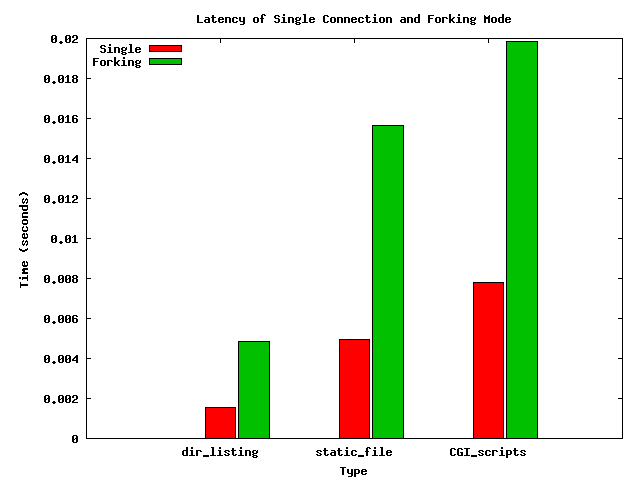
\includegraphics[width=4in,height=2.3in]{latency.png}
    \caption{Measuring latency of \textbf{spidey.py} with \textbf{thor.py}}
    \label{fig:my_label}
\end{figure}

\noindent The latency of handling the requests by forking is much longer than the latency of handling the requests by a single connection. When forking, an additional process (the child process) is created by the parent process. The creation of the child process, the copying the resources, and changing the identity child process, all of which is time consuming.


%-------------------------------------------------------

\section*{Throughput}
Throughput is how much data can be transferred in a given time. It is usually determined in bits/second. We decided to use thor.py and access files of size 1KB, 1MB, and 1 GB and measure the time taken. To create files of size 1KB, 1MB, and 1GB, we used the dd command to create random bytes. To measure the time taken, we used a shell script to access the 1KB and 1MB files 100 times, using 10 process and 10 requests in thor. Unfortunately, because the 1GB file was too large, we were only able to take a single sample. The results are shown in the following table and summarized in the following figure:
\begin{table}[H]
    \centering
    \begin{tabular}{|c||c|c|}
        \hline
        File Size & Single Connection  & Forking Mode  \\
        & (seconds) & (seconds) \\
        \hline
        \hline
         KB & 0.003149745 & 0.0129337947 \\
         MB & 2.36890281 & 2.222617403 \\
         GB & 2219.45399 & 2215.661636 \\
         \hline
    \end{tabular}
    \caption{Measuring Throughput of \textbf{spidey.py} with \textbf{thor.py}}
    \label{tab:my_label}
\end{table}
\begin{figure}[H]
    \centering
    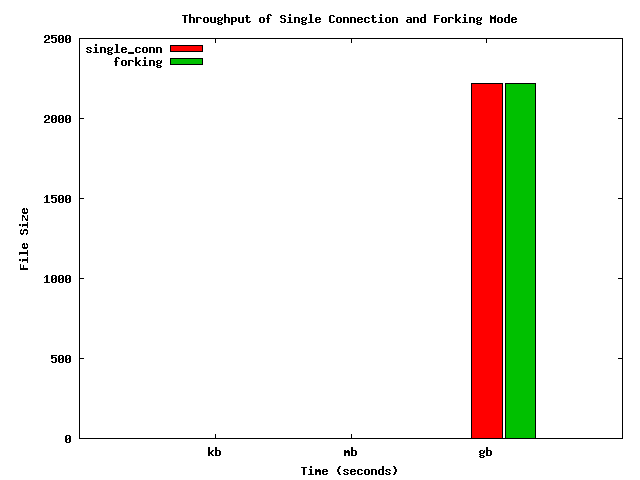
\includegraphics[width=4in, height=2.3in]{throughput.png}
    \caption{Average Throughput}
    \label{fig:my_label}
\end{figure}
\noindent The following is the shell scipt used to run the 1KB file 100 times:
\begin{verbatim}
        ./thor.py -p 10 -r 10 -v $URL/www/throughput/kilobyte 2>&1 > /dev/null 
        | grep "Average" | awk -F" " '{print &8}' >> throughput_kilo_test.txt' 
\end{verbatim}

\section*{Analysis}
The experiments show that for smaller requests, forking took more time. This is probably because forking requires time to create a child process, copy the parent's information, and change what the child is doing. However, for large requests, it seems like forking takes less time, especially if there are a large number of requests. However, overall the data seems to indicate that the difference in time taken is quite small. Forking also provides more benefits like being able to continue interacting with the UI while requests are going through, instead of waiting for each request to finish. Therefore, we believe that the forking model is more advantageous than the single connection model.

\section*{Conclusion}

Creating the HTTP client and the HTTP server furthered our understanding on how the web works. Networking is just sending and receiving packets of information. The client first sets up a socket, connects to the web server with an IP address and port, and sends a request for information to the web server.The web server also creates a socket, binds the socket to a public host and port, and listens for a request. When the web server receives a request from the client, it accepts the connections and does something with the client socket. \\

\noindent In creating web pages, we also learned basic HTML coding. We included an HTML5 audio element from YouTube to our 404 error page. By adding "?autoplay=1" to the end of the URL of the YouTube file, we were able to play the audio file automatically after the client receives information back from the server. \\

\noindent The assignment served as a review of material learned previously in class. It required us to use knowledge from the beginning of the semester, such as creating shell scripts to experiment with spidey.py and thor.py, revisiting the concept of latency, writing plt files, creating GNUplots, and writing in LATEX. 

\end{document}
